\chapter{Coherencia entre la métrica transcripcional y otros espacios de conocimiento (GO)}
En los capítulos precedentes cuantificamos por medio de diversos índices la congruencia biológica de los grupos encontrados en el espacio de expresión génica. En este capítulo buscaremos cuantificar la coherencia entre los espacios de expresión génica y de conocimiento biológico desde una óptica diferente: desde la métrica en lugar de desde las agrupaciones.
\section{Alineamiento de núcleo-objetivo}
Una matriz de núcleo o matriz de Gram o matriz de kernel $K$ puede ser pensada informalmente como una matriz de similaridad de a pares entre puntos de un conjunto de datos. Para un conjunto de datos $\{x_1,...,x_m\}$ esta similaridad depende de una función $k$ llamada kernel tal que:
\begin{equation}
	K = (k(x_i, x_j))_{i,j=1}^m
\end{equation}
Una función $k(x, y)$ es un kernel si y solo si para cualquier conjunto finito de datos $C=\{x_1,...,x_m\}$ y para cualquier conjunto $\{a_1,...,a_m\} \in \mathbb{R}^m$ se tiene que:
\begin{equation}
	\sum_{i,j=1}^m a_ia_jk(x_i, x_j)\geq 0
\end{equation}
Se puede demostrar que esto implica que $K$ debe ser semidefinida positiva (SDP), es decir, $K=\sum_i \lambda _i v_i v_i'$, con $\lambda _i \geq 0$ los autovalores de la matríz $K$ y $v_i$ sus autovectores.\\
Intuitivamente, un kernel es una transformación que mapea los puntos en un espacio de alta dimensionalidad a sus posiciones relativas mediante el uso de un producto interno.\\
Existen multiplicidad de kernerls disponibles y para cada aplicación será necesario encontrar el adecuado.\\
Es de esperar que si es posible extraer información biológica del espacio de expresión genética, entonces dos puntos que son similares (en algún sentido a definir por el kernel elegido) en el espacio de expresión, también lo sean en el espacio GO (nuevamente, en algún sentido a definir por el kernel elegido). Para cada espacio habrá que definir un kernel adecuado.\\
Una forma de cuantificar la similaridad entre estos dos espacios es mediante una cantidad conocida como alineamiento núcleo-objetivo o KTA. El KTA de un kernel $k_1$ con respecto a un kernel $k_2$ del conjunto $C$ esta definido como:
\begin{equation}
	\hat{A}(S, k_1, k_2) = \frac{\langle K_1, K_2 \rangle _F}{\sqrt{\langle K_1, K_1 \rangle _F \langle K_2, K_2 \rangle _F}}
\end{equation}
Donde $\langle K_1, K_1 \rangle _F = \sum_{i,j=1}^m K1(x_i, x_j)K2(x_i, x_j)$ es el producto de interno de Frobenius entre matrices y $K_i$ son las matrices de kernels simétricas y semidefinida positivas de los espacios a comparar. Este índice tiene un rango entre $[0, 1]$.\cite{Cristianini2006}\\
Es posible extender este concepto a matrices simétricas indefinidas (no SDP) $S$ mediante diversas técnicas que consisten en transformar $S$ para obtener una $S'$ SDP. La que utilizaremos en este trabajo se conoce como \textit{corrimiento del espectro}. Si $S$ es simétrica entonces admite una descomposición en autovalores y autovectores tal que $S=U\Lambda U^T$ con $U$ una matriz ortogonal y $\Lambda$ una matriz diagonal de autovalores reales, es decir, $\Lambda = diag(\lambda _1,...,\lambda _m)$. Entonces, el corrimiento del espectro consiste en correr todo el espectro de $S$ por el mínimo necesario: 
\begin{equation}
	S_{corrida} = U(\Lambda + |\min{\lambda _{min}(S), 0}|I)U^T 
	\label{eq:matriz_corrida}
\end{equation}
Decidimos utilizar este método porque el mismo solo aumenta las autosimilaridades, sin modificar la similaridad entre dos puntos distintos, preservando la estructura de grupo al agrupar datos no necesariamente métricos.\cite{Chen22009}\\
Notar que esta medida es una medida global, ya que toma en cuenta todas las similaridades para calcular KTA.\\
\section{Espacio de expresión y GO}
Para cuantificar la coherencia métrica entre el espacio de expresión de cada tratamiento y las ontologías GOBPA, GOBPB y GOCC, utilizamos como kernel de espacio de expresión, $K_x$, la similaridad derivada de la correlación:
\begin{equation}
	K_x = (\frac{correlacion(g_i, g_j)+1}{2})_{ij}
\end{equation}
con $g_i$ y $g_j$ genes pertenecientes al tratamiento en cuestión. Se puede demostrar que una matriz de similaridad definida de esta manera es siempre SDP.\\
Para el kernel del espacio de ontologías, utilizamos la similaridad definida en la ecuación \ref{eq:sim_rcmax} y transformamos la matriz en SDP por medio de \ref{eq:matriz_corrida}. La matriz se construyó tomando en cuenta todos los genes del tratamiento. Si un gen del tratamiento no se encontraba anotado en la ontología, se lo anotaba al nodo raíz y por lo tanto su similaridad con el resto de los genes era cero. Se calculó entonces para cada tratamiento y cada ontología, el KTA y se construyó además un control nulo de tipo 2, realizando 1000 reordenamientos aleatorios de las etiquetas de la matriz $K_x$.\\
Las figuras \ref{fig:kta_global} presentan un boxplot para cada tratamiento y cada ontología, con un punto rojo para el KTA de expresión y en negro, el KTA de control nulo. 
\begin{figure*}[t!]
    \centering
    \begin{subfigure}[t]{0.5\textwidth}
    \centering
    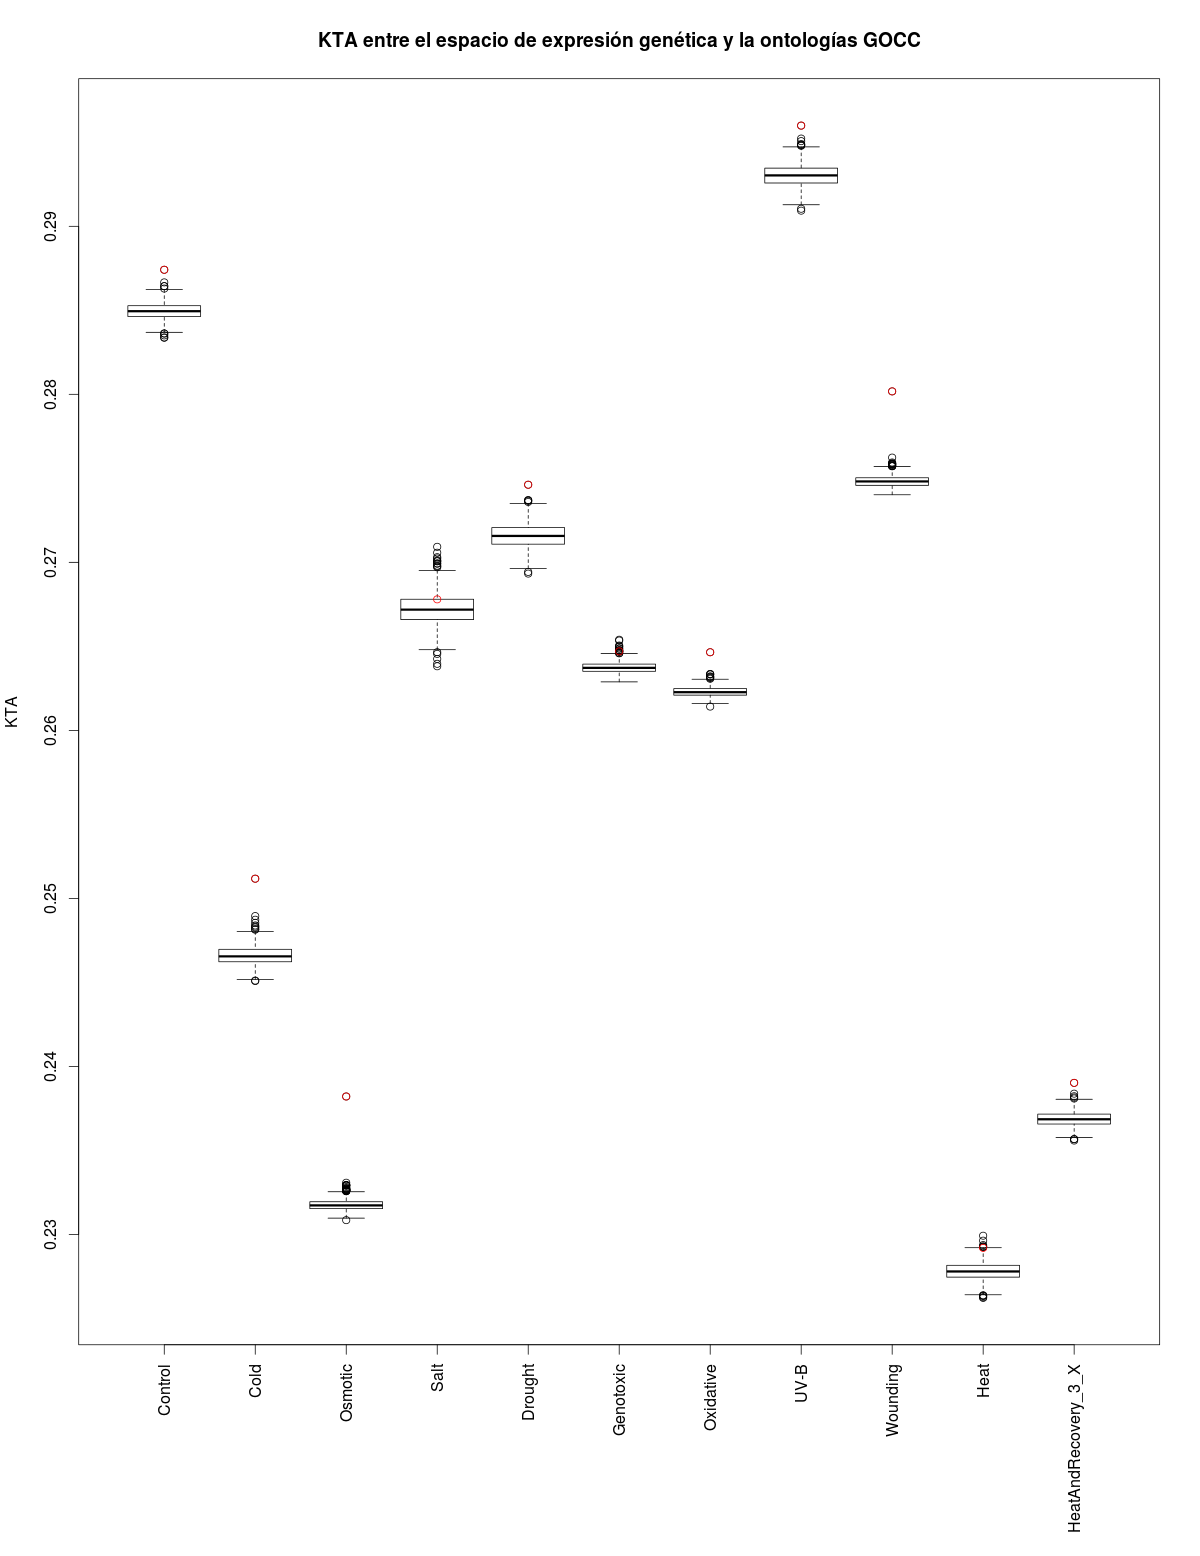
\includegraphics[width=1\textwidth]{kta_global_cc}
    \caption{KTA para ontología CC.}
    \end{subfigure}
    \begin{subfigure}[t]{0.5\textwidth}
    \centering
    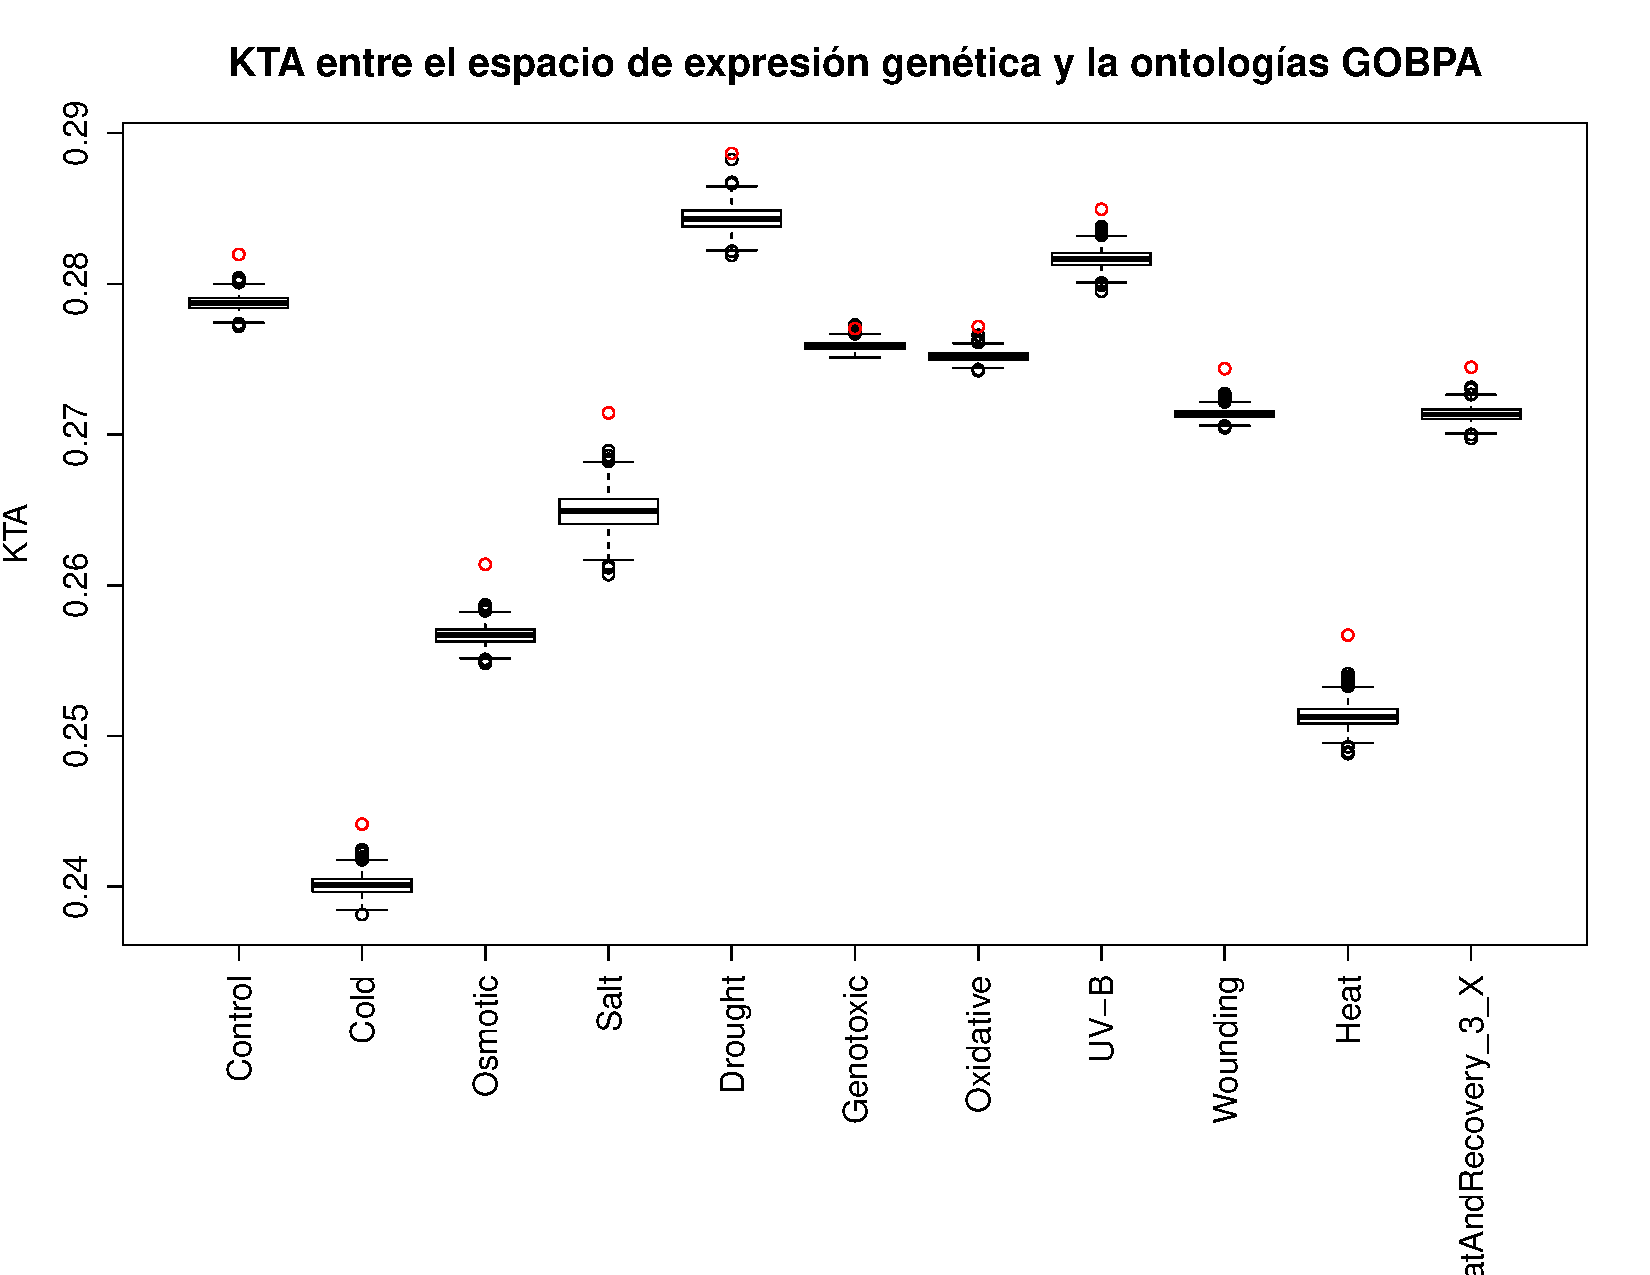
\includegraphics[width=1\textwidth]{kta_global_bpa}
    \caption{KTA para ontología BPA.}
    \end{subfigure}
    \begin{subfigure}[t]{0.5\textwidth}
    \centering
    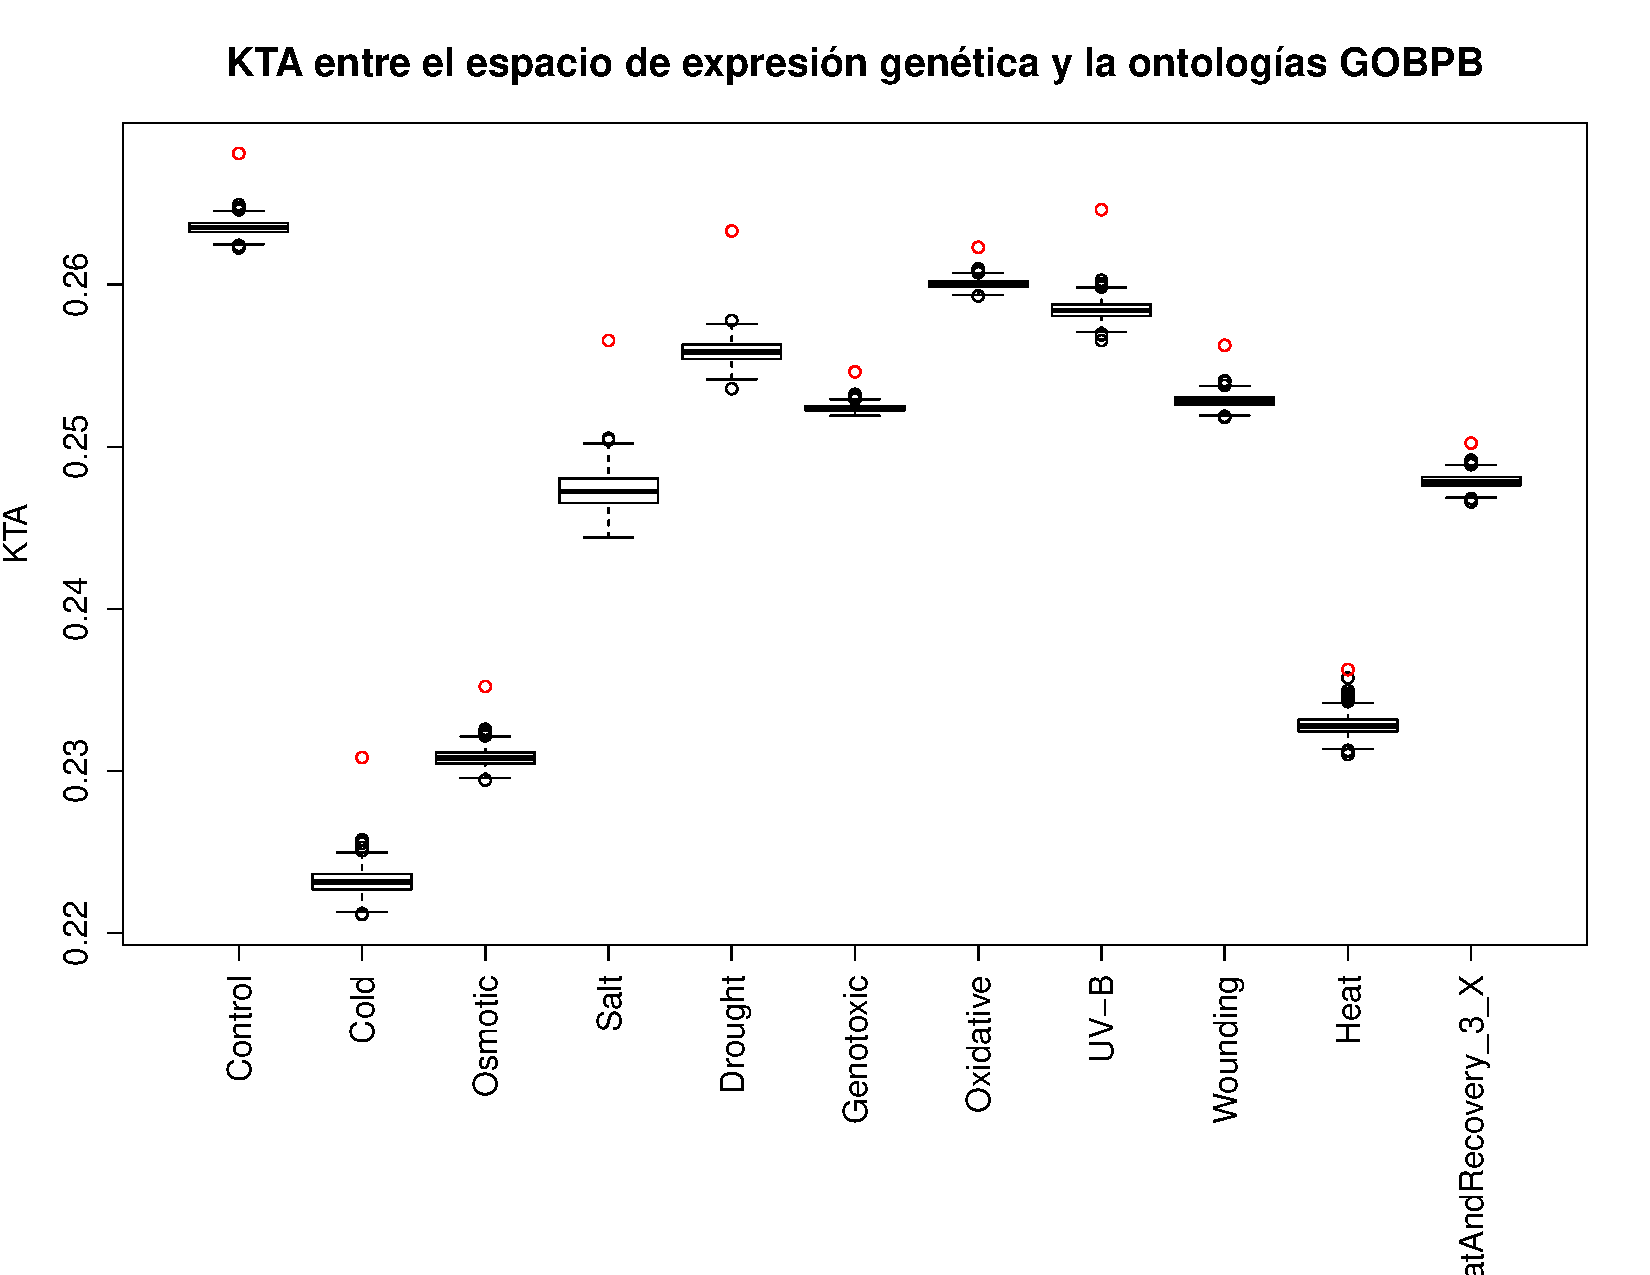
\includegraphics[width=1\textwidth]{kta_global_bpb}
    \caption{KTA para ontología BPB.}
    \end{subfigure}    
    \caption{Índice de alineamiento núcleo-objetivo, KTA, para distintos tratamientos entre espacio de expresión y espació de ontología.}
    \label{kta_global}
\end{figure*}
En todos los casos encontramos que el KTA de expresión supera todos los valores del KTA de control nulo, lo que indica una coherencia entre la métrica de expresión transcripcional y la métrica del espacio GO. \hl{completar las conclusiones un poco mas}.
\hl{zKTA: por tratamiento Gx/GOBPa, Gx/GOBPb, Gx/GOCC, Gx/PIN, Gx/LCI, Gx/Kegg}